\documentclass[a4paper,11pt]{article}
\usepackage[T1]{fontenc}
\usepackage[utf8]{inputenc}
\usepackage{lmodern}
\usepackage{textcomp}
\usepackage{amssymb}
\usepackage[margin=1.5cm]{geometry}
\usepackage{lscape}

\title{HICF1 -  Final Report v4}
\author{Dr. Susanne Weller}
\date{\today}

\usepackage{Sweave}
\begin{document}
\input{HICF1_Finalreportv4-concordance}

\maketitle
\tableofcontents
\section{Univariate Analysis}
Note that TP53\_mut are only mutation with >5\%VAF! Univariate p-values change dramatically if you add more variables, this is due to the multiple testing problem. I have used False Discovery Rate, currently the least stringent correction method that was specifically designed for genetics.

% Table created by stargazer v.5.1 by Marek Hlavac, Harvard University. E-mail: hlavac at fas.harvard.edu
% Date and time: Wed, Aug 06, 2014 - 16:19:01
\begin{table}[!htbp] \centering 
  \caption{Univariate Analysis against MRD outcome} 
  \label{} 
\tiny 
\begin{tabular}{@{\extracolsep{0p}} ccccccccc} 
\\[-1.8ex]\hline 
\hline \\[-1.8ex] 
 & p & sig & corr.p & sig.corr & MRDpos\_0 & MRDneg\_0 & MRDpos\_1 & MRDneg\_1 \\ 
\hline \\[-1.8ex] 
ATM\_ALL & $0.002$ & \textasteriskcentered \textasteriskcentered  & $0.005$ & \textasteriskcentered \textasteriskcentered  & 28\% & 40\% & 21\% & 11\% \\ 
ATM\_bi & $0.002$ & \textasteriskcentered \textasteriskcentered  & $0.005$ & \textasteriskcentered \textasteriskcentered  & 40\% & 49\% & 9\% & 2\% \\ 
ATM\_del & $0$ & \textasteriskcentered \textasteriskcentered \textasteriskcentered  & $0$ & \textasteriskcentered \textasteriskcentered \textasteriskcentered  & 35\% & 47\% & 13\% & 4\% \\ 
ATM\_mono & $0.836$ & n.s. & $0.836$ & n.s. & 43\% & 44\% & 6\% & 7\% \\ 
BIRC3\_ALL & $0.095$ & trend & $0.129$ & n.s. & 38\% & 45\% & 11\% & 6\% \\ 
BIRC3\_bi & $0.360$ & n.s. & $0.428$ & n.s. & 47\% & 51\% & 1\% & 0\% \\ 
BIRC3\_del & $0.002$ & \textasteriskcentered \textasteriskcentered  & $0.005$ & \textasteriskcentered \textasteriskcentered  & 39\% & 48\% & 10\% & 3\% \\ 
BIRC3\_mono & $0.066$ & trend & $0.101$ & n.s. & 48\% & 48\% & 0\% & 3\% \\ 
NOTCH1\_mut & $0.069$ & trend & $0.101$ & n.s. & 44\% & 42\% & 4\% & 9\% \\ 
SAMHD1\_ALL & $0.054$ & trend & $0.093$ & trend & 45\% & 50\% & 4\% & 1\% \\ 
SF3B1\_mut & $0.415$ & n.s. & $0.464$ & n.s. & 36\% & 41\% & 12\% & 11\% \\ 
TP53\_ALL & $0$ & \textasteriskcentered \textasteriskcentered \textasteriskcentered  & $0$ & \textasteriskcentered \textasteriskcentered \textasteriskcentered  & 40\% & 50\% & 9\% & 1\% \\ 
TP53\_bi & $0.009$ & \textasteriskcentered \textasteriskcentered  & $0.021$ & \textasteriskcentered  & 44\% & 51\% & 4\% & 0\% \\ 
TP53\_lowVAF & $0.163$ & n.s. & $0.206$ & n.s. & 46\% & 50\% & 3\% & 1\% \\ 
TP53\_mut & $0$ & \textasteriskcentered \textasteriskcentered \textasteriskcentered  & $0$ & \textasteriskcentered \textasteriskcentered \textasteriskcentered  & 42\% & 51\% & 7\% & 0\% \\ 
Trisomy\_12 & $0.002$ & \textasteriskcentered \textasteriskcentered  & $0.005$ & \textasteriskcentered \textasteriskcentered  & 45\% & 39\% & 4\% & 12\% \\ 
X11q\_mono & $0.046$ & \textasteriskcentered  & $0.093$ & trend & 44\% & 50\% & 5\% & 1\% \\ 
Subclones & $0.050$ & \textasteriskcentered  & $0.093$ & trend & NA\% & NA\% & NA\% & NA\% \\ 
Total\_num\_CNAs & $0.483$ & n.s. & $0.510$ & n.s. & NA\% & NA\% & NA\% & NA\% \\ 
\hline \\[-1.8ex] 
\end{tabular} 
\end{table} 
\section{Associations}
To test for associations, I first counted the number of patients that have a particular mutation, and derived the probablity of having this lesion:\\
Example:\\
8 out of 209 patients have mutation X -> probability estimate for this mutation is 8/209\\
15 out of 209 patients have mutation Y ->  probability estimate for this mutation is 15/209\\
The expected probablity of having both mutations is then 8/209 x 15/209\\

I then compared this expected probability to the observed probability using Exact Binomial Tests. This test is the only one that I could find that can deal with low numbers AND allows for testing agains expected frequencies. Fisher's Exact test is often used that way by constructing the expected frequencies from the expected probabilities, but does not allow for integers, which is a problem with the low numbers we are dealing with.\\
I again used False Discovery Rate to correct the p-values.



\begin{landscape}
% latex table generated in R 3.0.1 by xtable 1.7-3 package
% Wed Aug  6 16:19:02 2014
\begin{table}[ht]
\centering
{\tiny
\scalebox{0.6}{
\begin{tabular}{|r|c|c|c|c|c|c|c|c|c|c|c|c|c|c|c|c|c|c|c|c|c|c|c|c|c|}
  \hline
variables & TP53\_ALL & TP53\_del & TP53\_cnLOH & TP53\_mut & ATM\_ALL & ATM\_mut & ATM\_del & ATM\_cnLOH & BIRC3\_ALL & BIRC3\_mut & BIRC3\_del & NOTCH1\_mut & SF3B1\_mut & X6q.\_del\_ALL & X13q\_ALL & Trisomy\_12 & Trisomy\_18 & Trisomy\_19 & XPO1\_gain & SAMHD1\_ALL & MYD88\_mut & MED12mutation & X8q\_ALL & Subclones & Total\_num\_CNAs \\ 
  \hline
TP53\_ALL &  & 0.00 & 0.00 & 0.00 & 0.00 & 0.51 & 0.57 & 0.50 & 1.00 & 0.41 & 0.34 & 1.00 & 0.59 & 0.39 & 0.44 & 1.00 & 0.63 & 0.64 & 0.43 & 0.42 & 0.10 & 0.69 & 0.08 & 0.66 & 0.07 \\ 
  TP53\_del &  &  & 1.00 & 0.00 & 0.00 & 0.27 & 0.53 & 0.43 & 1.00 & 1.00 & 0.42 & 1.00 & 0.64 & 0.63 & 1.00 & 1.00 & 0.67 & 1.00 & 0.65 & 0.18 & 0.47 & 0.82 & 0.63 & 1.00 & 0.18 \\ 
  TP53\_cnLOH &  &  &  & 0.01 & 0.00 & 1.00 & 0.63 & 0.51 & 1.00 & 1.00 & 1.00 & 1.00 & 1.00 & 1.00 & 1.00 & 0.21 & 1.00 & 1.00 & 0.10 & 0.60 & 1.00 & 0.17 & 1.00 & 0.09 & 0.61 \\ 
  TP53\_mut &  &  &  &  & 0.00 & 0.17 & 0.19 & 0.28 & 1.00 & 0.63 & 0.09 & 0.64 & 0.19 & 0.18 & 1.00 & 1.00 & 1.00 & 1.00 & 1.00 & 1.00 & 0.36 & 0.88 & 0.18 & 0.38 & 0.10 \\ 
  ATM\_ALL &  &  &  &  &  & 0.64 & 0.59 & 0.53 & 1.00 & 0.51 & 0.18 & 1.00 & 0.43 & 0.42 & 1.00 & 0.56 & 0.48 & 1.00 & 1.00 & 0.39 & 0.58 & 1.00 & 0.42 & 0.54 & 0.39 \\ 
  ATM\_mut &  &  &  &  &  &  & 0.00 & 0.00 & 0.03 & 0.00 & 0.00 & 0.37 & 0.00 & 0.00 & 0.03 & 0.00 & 0.00 & 0.59 & 0.44 & 0.55 & 0.66 & 0.80 & 0.74 & 0.85 & 0.19 \\ 
  ATM\_del &  &  &  &  &  &  &  & 0.00 & 0.01 & 0.00 & 0.11 & 0.20 & 0.02 & 0.00 & 0.65 & 0.06 & 0.00 & 0.53 & 0.16 & 0.58 & 0.60 & 0.52 & 0.25 & 0.92 & 0.35 \\ 
  ATM\_cnLOH &  &  &  &  &  &  &  &  & 1.00 & 0.28 & 0.00 & 0.02 & 0.00 & 0.00 & 0.00 & 0.00 & 0.00 & 0.70 & 0.83 & 0.40 & 0.34 & 1.00 & 0.34 & 0.54 & 0.19 \\ 
  BIRC3\_ALL &  &  &  &  &  &  &  &  &  & 1.00 & 1.00 & 1.00 & 1.00 & 0.00 & 1.00 & 1.00 & 1.00 & 1.00 & 1.00 & 0.31 & 1.00 & 0.35 & 0.43 & 0.47 & 1.00 \\ 
  BIRC3\_mut &  &  &  &  &  &  &  &  &  &  & 0.28 & 1.00 & 0.41 & 0.65 & 1.00 & 1.00 & 0.00 & 1.00 & 1.00 & 0.35 & 1.00 & 0.54 & 0.39 & 0.65 & 0.07 \\ 
  BIRC3\_del &  &  &  &  &  &  &  &  &  &  &  & 0.00 & 0.00 & 0.00 & 0.00 & 0.00 & 0.00 & 0.00 & 0.66 & 1.00 & 0.74 & 0.82 & 0.34 & 0.71 & 0.51 \\ 
  NOTCH1\_mut &  &  &  &  &  &  &  &  &  &  &  &  & 0.04 & 1.00 & 0.00 & 1.00 & 0.18 & 0.00 & 0.05 & 1.00 & 0.61 & 0.86 & 1.00 & 1.00 & 1.00 \\ 
  SF3B1\_mut &  &  &  &  &  &  &  &  &  &  &  &  &  & 0.00 & 0.00 & 0.00 & 0.02 & 0.64 & 0.45 & 0.84 & 0.71 & 0.90 & 0.27 & 0.66 & 0.44 \\ 
  X6q.\_del\_ALL &  &  &  &  &  &  &  &  &  &  &  &  &  &  & 1.00 & 0.42 & 0.03 & 1.00 & 0.59 & 0.22 & 0.24 & 0.50 & 1.00 & 0.45 & 0.42 \\ 
  X13q\_ALL &  &  &  &  &  &  &  &  &  &  &  &  &  &  &  & 1.00 & 1.00 & 1.00 & 0.49 & 1.00 & 1.00 & 1.00 & 1.00 & 1.00 & 1.00 \\ 
  Trisomy\_12 &  &  &  &  &  &  &  &  &  &  &  &  &  &  &  &  & 0.29 & 1.00 & 0.71 & 0.56 & 0.58 & 1.00 & 0.42 & 0.54 & 0.15 \\ 
  Trisomy\_18 &  &  &  &  &  &  &  &  &  &  &  &  &  &  &  &  &  & 0.41 & 0.25 & 0.86 & 1.00 & 0.91 & 0.21 & 0.60 & 0.60 \\ 
  Trisomy\_19 &  &  &  &  &  &  &  &  &  &  &  &  &  &  &  &  &  &  & 0.05 & 1.00 & 0.47 & 1.00 & 1.00 & 1.00 & 1.00 \\ 
  XPO1\_gain &  &  &  &  &  &  &  &  &  &  &  &  &  &  &  &  &  &  &  & 0.13 & 0.73 & 0.08 & 0.28 & 0.26 & 0.46 \\ 
  SAMHD1\_ALL &  &  &  &  &  &  &  &  &  &  &  &  &  &  &  &  &  &  &  &  & 0.16 & 0.84 & 0.54 & 0.44 & 0.14 \\ 
  MYD88\_mut &  &  &  &  &  &  &  &  &  &  &  &  &  &  &  &  &  &  &  &  &  & 1.00 & 1.00 & 0.69 & 1.00 \\ 
  MED12mutation &  &  &  &  &  &  &  &  &  &  &  &  &  &  &  &  &  &  &  &  &  &  & 0.00 & 0.00 & 0.00 \\ 
  X8q\_ALL &  &  &  &  &  &  &  &  &  &  &  &  &  &  &  &  &  &  &  &  &  &  &  & 0.00 & 0.15 \\ 
  Subclones &  &  &  &  &  &  &  &  &  &  &  &  &  &  &  &  &  &  &  &  &  &  &  &  & 0.00 \\ 
  Total\_num\_CNAs &  &  &  &  &  &  &  &  &  &  &  &  &  &  &  &  &  &  &  &  &  &  &  &  &  \\ 
   \hline
\end{tabular}
}
}
\caption{Association chart, uncorrected pvalues, Fisher's test} 
\end{table}
% latex table generated in R 3.0.1 by xtable 1.7-3 package
% Wed Aug  6 16:19:02 2014
\begin{table}[ht]
\centering
{\tiny
\scalebox{0.6}{
\begin{tabular}{|r|c|c|c|c|c|c|c|c|c|c|c|c|c|c|c|c|c|c|c|c|c|c|c|c|c|}
  \hline
variables & TP53\_ALL & TP53\_del & TP53\_cnLOH & TP53\_mut & ATM\_ALL & ATM\_mut & ATM\_del & ATM\_cnLOH & BIRC3\_ALL & BIRC3\_mut & BIRC3\_del & NOTCH1\_mut & SF3B1\_mut & X6q.\_del\_ALL & X13q\_ALL & Trisomy\_12 & Trisomy\_18 & Trisomy\_19 & XPO1\_gain & SAMHD1\_ALL & MYD88\_mut & MED12mutation & X8q\_ALL & Subclones & Total\_num\_CNAs \\ 
  \hline
TP53\_ALL &  & 0.00 & 0.01 & 0.00 & 0.00 & 1.00 & 1.00 & 1.00 & 1.00 & 0.99 & 0.98 & 1.00 & 1.00 & 0.99 & 0.99 & 1.00 & 1.00 & 1.00 & 0.99 & 0.99 & 0.46 & 1.00 & 0.41 & 1.00 & 0.37 \\ 
  TP53\_del &  &  & 1.00 & 0.00 & 0.00 & 0.85 & 1.00 & 0.99 & 1.00 & 1.00 & 0.99 & 1.00 & 1.00 & 1.00 & 1.00 & 1.00 & 1.00 & 1.00 & 1.00 & 0.68 & 1.00 & 1.00 & 1.00 & 1.00 & 0.68 \\ 
  TP53\_cnLOH &  &  &  & 0.03 & 0.01 & 1.00 & 1.00 & 1.00 & 1.00 & 1.00 & 1.00 & 1.00 & 1.00 & 1.00 & 1.00 & 0.71 & 1.00 & 1.00 & 0.46 & 1.00 & 1.00 & 0.68 & 1.00 & 0.43 & 1.00 \\ 
  TP53\_mut &  &  &  &  & 0.00 & 0.68 & 0.68 & 0.85 & 1.00 & 1.00 & 0.42 & 1.00 & 0.68 & 0.68 & 1.00 & 1.00 & 1.00 & 1.00 & 1.00 & 1.00 & 0.98 & 1.00 & 0.68 & 0.99 & 0.46 \\ 
  ATM\_ALL &  &  &  &  &  & 1.00 & 1.00 & 1.00 & 1.00 & 1.00 & 0.68 & 1.00 & 0.99 & 0.99 & 1.00 & 1.00 & 1.00 & 1.00 & 1.00 & 0.99 & 1.00 & 1.00 & 0.99 & 1.00 & 0.99 \\ 
  ATM\_mut &  &  &  &  &  &  & 0.00 & 0.00 & 0.18 & 0.01 & 0.00 & 0.99 & 0.00 & 0.00 & 0.18 & 0.00 & 0.00 & 1.00 & 0.99 & 1.00 & 1.00 & 1.00 & 1.00 & 1.00 & 0.68 \\ 
  ATM\_del &  &  &  &  &  &  &  & 0.02 & 0.07 & 0.00 & 0.50 & 0.69 & 0.10 & 0.00 & 1.00 & 0.30 & 0.00 & 1.00 & 0.65 & 1.00 & 1.00 & 1.00 & 0.82 & 1.00 & 0.98 \\ 
  ATM\_cnLOH &  &  &  &  &  &  &  &  & 1.00 & 0.86 & 0.00 & 0.11 & 0.00 & 0.00 & 0.01 & 0.00 & 0.02 & 1.00 & 1.00 & 0.99 & 0.98 & 1.00 & 0.98 & 1.00 & 0.68 \\ 
  BIRC3\_ALL &  &  &  &  &  &  &  &  &  & 1.00 & 1.00 & 1.00 & 1.00 & 0.00 & 1.00 & 1.00 & 1.00 & 1.00 & 1.00 & 0.93 & 1.00 & 0.98 & 0.99 & 1.00 & 1.00 \\ 
  BIRC3\_mut &  &  &  &  &  &  &  &  &  &  & 0.85 & 1.00 & 0.99 & 1.00 & 1.00 & 1.00 & 0.00 & 1.00 & 1.00 & 0.98 & 1.00 & 1.00 & 0.99 & 1.00 & 0.34 \\ 
  BIRC3\_del &  &  &  &  &  &  &  &  &  &  &  & 0.00 & 0.00 & 0.00 & 0.01 & 0.00 & 0.02 & 0.00 & 1.00 & 1.00 & 1.00 & 1.00 & 0.98 & 1.00 & 1.00 \\ 
  NOTCH1\_mut &  &  &  &  &  &  &  &  &  &  &  &  & 0.23 & 1.00 & 0.00 & 1.00 & 0.68 & 0.00 & 0.28 & 1.00 & 1.00 & 1.00 & 1.00 & 1.00 & 1.00 \\ 
  SF3B1\_mut &  &  &  &  &  &  &  &  &  &  &  &  &  & 0.00 & 0.00 & 0.00 & 0.10 & 1.00 & 0.99 & 1.00 & 1.00 & 1.00 & 0.85 & 1.00 & 0.99 \\ 
  X6q.\_del\_ALL &  &  &  &  &  &  &  &  &  &  &  &  &  &  & 1.00 & 0.99 & 0.15 & 1.00 & 1.00 & 0.73 & 0.80 & 1.00 & 1.00 & 0.99 & 0.99 \\ 
  X13q\_ALL &  &  &  &  &  &  &  &  &  &  &  &  &  &  &  & 1.00 & 1.00 & 1.00 & 1.00 & 1.00 & 1.00 & 1.00 & 1.00 & 1.00 & 1.00 \\ 
  Trisomy\_12 &  &  &  &  &  &  &  &  &  &  &  &  &  &  &  &  & 0.86 & 1.00 & 1.00 & 1.00 & 1.00 & 1.00 & 0.99 & 1.00 & 0.64 \\ 
  Trisomy\_18 &  &  &  &  &  &  &  &  &  &  &  &  &  &  &  &  &  & 0.99 & 0.82 & 1.00 & 1.00 & 1.00 & 0.71 & 1.00 & 1.00 \\ 
  Trisomy\_19 &  &  &  &  &  &  &  &  &  &  &  &  &  &  &  &  &  &  & 0.25 & 1.00 & 1.00 & 1.00 & 1.00 & 1.00 & 1.00 \\ 
  XPO1\_gain &  &  &  &  &  &  &  &  &  &  &  &  &  &  &  &  &  &  &  & 0.57 & 1.00 & 0.39 & 0.85 & 0.84 & 1.00 \\ 
  SAMHD1\_ALL &  &  &  &  &  &  &  &  &  &  &  &  &  &  &  &  &  &  &  &  & 0.66 & 1.00 & 1.00 & 0.99 & 0.63 \\ 
  MYD88\_mut &  &  &  &  &  &  &  &  &  &  &  &  &  &  &  &  &  &  &  &  &  & 1.00 & 1.00 & 1.00 & 1.00 \\ 
  MED12mutation &  &  &  &  &  &  &  &  &  &  &  &  &  &  &  &  &  &  &  &  &  &  & 0.01 & 0.00 & 0.00 \\ 
  X8q\_ALL &  &  &  &  &  &  &  &  &  &  &  &  &  &  &  &  &  &  &  &  &  &  &  & 0.00 & 0.64 \\ 
  Subclones &  &  &  &  &  &  &  &  &  &  &  &  &  &  &  &  &  &  &  &  &  &  &  &  & 0.00 \\ 
  Total\_num\_CNAs &  &  &  &  &  &  &  &  &  &  &  &  &  &  &  &  &  &  &  &  &  &  &  &  &  \\ 
   \hline
\end{tabular}
}
}
\caption{Association chart, corrected pvalues, Fisher's test with FDR correction} 
\end{table} \end{landscape}

Odds ratios and p-values for associations between genes are represented in this heatmap. Note that odds ratios 0-1 (the first bar in the colour key) are mutually exclusive, everything else already counts as co-occuring.\\
\emph{Note: Colour key still needs be adjusted to a somewhat funny scale to see this properly.}

\begin{landscape}
% latex table generated in R 3.0.1 by xtable 1.7-3 package
% Wed Aug  6 16:19:02 2014
\begin{table}[ht]
\centering
{\tiny
\scalebox{0.6}{
\begin{tabular}{|r|c|c|c|c|c|c|c|c|c|c|c|c|c|c|c|c|c|c|c|c|c|c|c|c|c|}
  \hline
variables & TP53\_ALL & TP53\_del & TP53\_cnLOH & TP53\_mut & ATM\_ALL & ATM\_mut & ATM\_del & ATM\_cnLOH & BIRC3\_ALL & BIRC3\_mut & BIRC3\_del & NOTCH1\_mut & SF3B1\_mut & X6q.\_del\_ALL & X13q\_ALL & Trisomy\_12 & Trisomy\_18 & Trisomy\_19 & XPO1\_gain & SAMHD1\_ALL & MYD88\_mut & MED12mutation & X8q\_ALL & Subclones & Total\_num\_CNAs \\ 
  \hline
TP53\_ALL &  & 8.86 & 8.66 & 9.22 & 9.00 & 0.71 & 0.67 & 0.60 & 0.00 & 1.43 & 0.42 & 0.57 & 0.57 & 0.31 & 1.71 & 0.61 & 1.16 & 0.00 & 1.34 & 1.27 & 2.30 & 0.86 & 0.00 & 1.10 & 0.30 \\ 
  TP53\_del &  &  & 0.00 & 12.43 & 17.77 & 0.28 & 0.38 & 0.00 & 0.00 & 0.00 & 0.00 & 0.00 & 0.00 & 0.00 & 0.00 & 0.00 & 1.29 & 0.00 & 0.00 & 0.00 & 1.60 & 0.74 & 0.00 & 0.95 & 0.00 \\ 
  TP53\_cnLOH &  &  &  & 9.06 & 12.95 & 0.72 & 0.00 & 1.42 & 0.00 & 0.00 & 0.00 & 0.00 & 0.00 & 0.00 & 0.00 & 4.28 & 0.00 & 0.00 & 3.76 & 1.11 & 0.00 & 1.88 & 0.00 & 2.39 & 1.07 \\ 
  TP53\_mut &  &  &  &  & 11.68 & 0.42 & 0.37 & 0.28 & 0.00 & 0.00 & 0.00 & 0.00 & 0.00 & 0.00 & 0.00 & 0.85 & 0.97 & 0.00 & 0.74 & 0.88 & 1.60 & 1.03 & 0.00 & 1.32 & 0.21 \\ 
  ATM\_ALL &  &  &  &  &  & 0.61 & 0.54 & 0.40 & 0.00 & 1.42 & 0.00 & 0.00 & 0.00 & 0.00 & 0.00 & 1.22 & 1.39 & 0.00 & 0.53 & 0.31 & 1.14 & 0.93 & 0.00 & 1.19 & 0.30 \\ 
  ATM\_mut &  &  &  &  &  &  & 3.55 & 3.28 & 2.92 & 2.98 & 2.51 & 1.35 & 3.15 & 3.12 & 2.92 & 3.00 & 3.12 & 0.57 & 0.71 & 1.13 & 1.16 & 1.04 & 1.07 & 1.03 & 1.32 \\ 
  ATM\_del &  &  &  &  &  &  &  & 2.09 & 3.85 & 3.94 & 1.55 & 0.25 & 1.96 & 4.15 & 0.00 & 0.00 & 4.17 & 0.38 & 0.47 & 1.13 & 1.27 & 1.11 & 1.42 & 1.02 & 1.24 \\ 
  ATM\_cnLOH &  &  &  &  &  &  &  &  & 0.00 & 0.00 & 5.10 & 2.71 & 6.36 & 5.01 & 5.79 & 5.98 & 0.00 & 1.14 & 1.07 & 1.28 & 1.53 & 0.98 & 0.42 & 1.14 & 1.45 \\ 
  BIRC3\_ALL &  &  &  &  &  &  &  &  &  & 0.00 & 0.00 & 0.00 & 0.00 & 9.02 & 0.00 & 0.00 & 0.00 & 0.00 & 0.00 & 1.78 & 0.00 & 1.50 & 1.77 & 1.43 & 0.85 \\ 
  BIRC3\_mut &  &  &  &  &  &  &  &  &  &  & 0.00 & 0.00 & 0.00 & 0.00 & 0.00 & 0.00 & 6.75 & 0.00 & 0.62 & 1.48 & 0.00 & 1.25 & 1.48 & 1.19 & 2.16 \\ 
  BIRC3\_del &  &  &  &  &  &  &  &  &  &  &  & 6.31 & 6.69 & 3.72 & 6.08 & 4.41 & 0.00 & 6.19 & 1.12 & 1.00 & 1.20 & 0.93 & 0.44 & 1.07 & 1.18 \\ 
  NOTCH1\_mut &  &  &  &  &  &  &  &  &  &  &  &  & 2.69 & 0.59 & 16.25 & 0.00 & 0.00 & 16.59 & 2.52 & 0.88 & 1.06 & 0.87 & 0.59 & 0.95 & 0.85 \\ 
  SF3B1\_mut &  &  &  &  &  &  &  &  &  &  &  &  &  & 4.66 & 8.12 & 5.90 & 0.00 & 0.00 & 0.49 & 1.03 & 1.06 & 0.93 & 0.29 & 1.11 & 1.29 \\ 
  X6q.\_del\_ALL &  &  &  &  &  &  &  &  &  &  &  &  &  &  & 0.00 & 0.00 & 0.00 & 0.88 & 0.55 & 1.49 & 1.78 & 1.19 & 0.98 & 1.24 & 1.27 \\ 
  X13q\_ALL &  &  &  &  &  &  &  &  &  &  &  &  &  &  &  & 0.00 & 0.00 & 0.00 & 1.50 & 0.88 & 0.00 & 0.74 & 0.00 & 0.95 & 0.85 \\ 
  Trisomy\_12 &  &  &  &  &  &  &  &  &  &  &  &  &  &  &  &  & 0.00 & 0.00 & 1.07 & 1.27 & 1.14 & 0.93 & 0.00 & 1.19 & 1.85 \\ 
  Trisomy\_18 &  &  &  &  &  &  &  &  &  &  &  &  &  &  &  &  &  & 0.00 & 0.40 & 0.83 & 0.86 & 1.01 & 1.70 & 0.82 & 1.16 \\ 
  Trisomy\_19 &  &  &  &  &  &  &  &  &  &  &  &  &  &  &  &  &  &  & 3.02 & 0.88 & 1.60 & 0.93 & 0.88 & 0.95 & 0.85 \\ 
  XPO1\_gain &  &  &  &  &  &  &  &  &  &  &  &  &  &  &  &  &  &  &  & 0.41 & 0.50 & 0.57 & 0.27 & 0.65 & 0.66 \\ 
  SAMHD1\_ALL &  &  &  &  &  &  &  &  &  &  &  &  &  &  &  &  &  &  &  &  & 1.79 & 1.04 & 0.65 & 1.16 & 1.46 \\ 
  MYD88\_mut &  &  &  &  &  &  &  &  &  &  &  &  &  &  &  &  &  &  &  &  &  & 1.00 & 0.59 & 1.11 & 0.85 \\ 
  MED12mutation &  &  &  &  &  &  &  &  &  &  &  &  &  &  &  &  &  &  &  &  &  &  & 1.98 & 2.50 & 2.13 \\ 
  X8q\_ALL &  &  &  &  &  &  &  &  &  &  &  &  &  &  &  &  &  &  &  &  &  &  &  & 0.00 & 1.61 \\ 
  Subclones &  &  &  &  &  &  &  &  &  &  &  &  &  &  &  &  &  &  &  &  &  &  &  &  & 2.17 \\ 
  Total\_num\_CNAs &  &  &  &  &  &  &  &  &  &  &  &  &  &  &  &  &  &  &  &  &  &  &  &  &  \\ 
   \hline
\end{tabular}
}
}
\caption{Odds ratios for association between genes} 
\end{table}\end{landscape}
\newpage

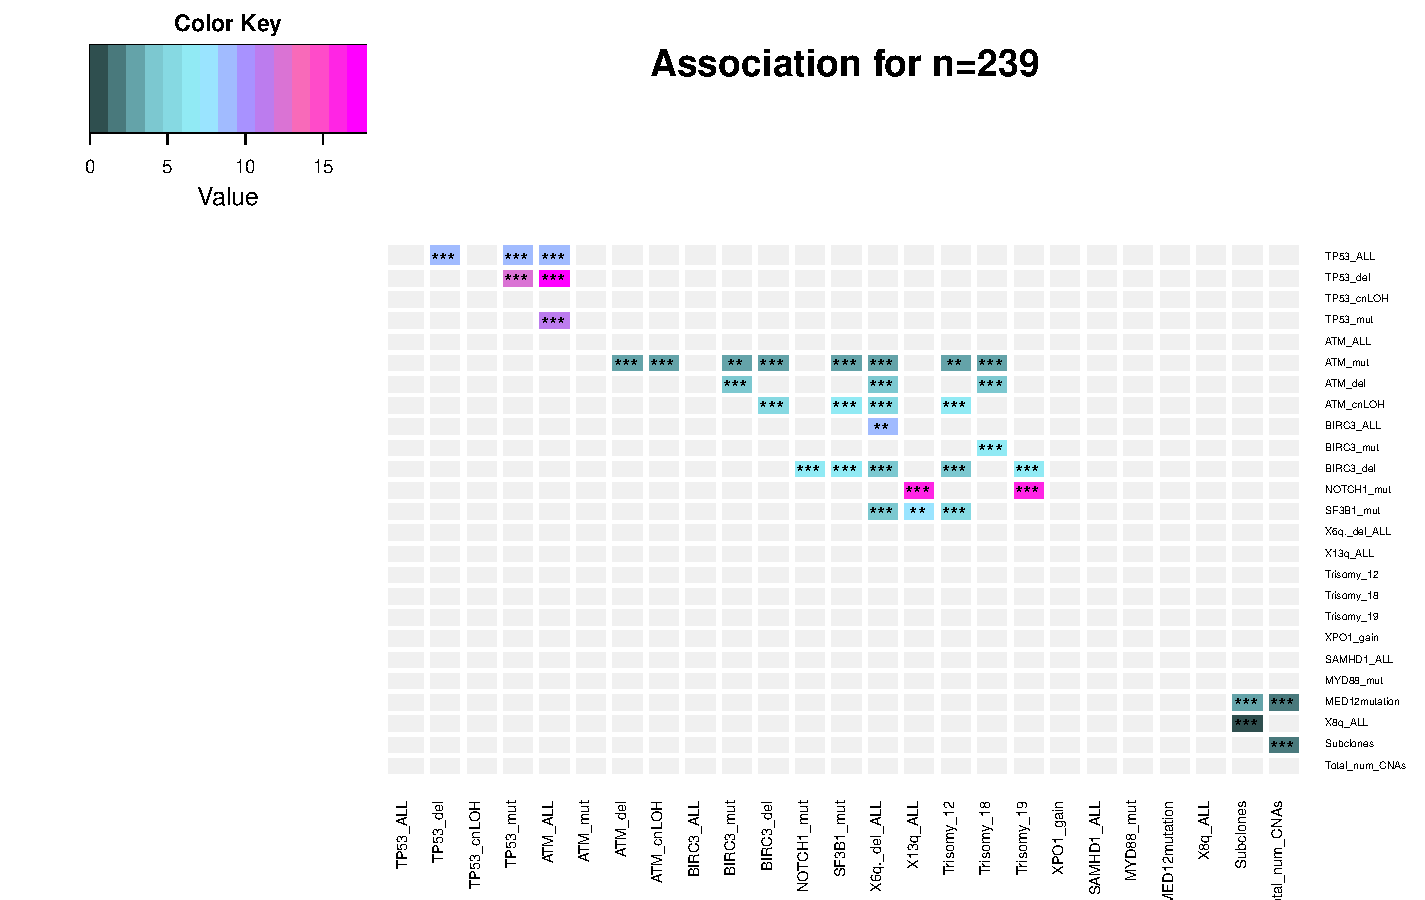
\includegraphics{HICF1_Finalreportv4-009}
\section{Model building - from here, only 209 data points will be used}
% \section{Association on model data}
% This was calculated to see if there are Co-linearities that have to be taken into account for the modelling. There are fewer associations than in the 239 data set, but as you can see from the chart, the associations don't change much.
% <<Model data set, echo=FALSE, eval=TRUE>>=
% model.genclinv6 <-subset(genclinv6, !is.na(genclinv6$MRD))
% #These are the variables that we want for the association chart
% variables_ass <- c("TP53_ALL", "TP53_mut", "TP53_del", "TP53_cnLOH", "ATM_ALL", "ATM_mut", "ATM_del", "ATM_cnLOH", "BIRC3_ALL", "BIRC3_mut", "BIRC3_del", "NOTCH1_mut", "SF3B1_mut", "X13q_ALL", "X6q._del_ALL", "Trisomy_12", "Trisomy_18", "Trisomy_19", "XPO1_gain", "SAMHD1_ALL", "MYD88_mut", "MED12mutation", "X8q_ALL", "Subclones", "Total_num_CNAs")
% model.genclinv6.ass <- model.genclinv6[colnames(model.genclinv6) %in% variables_ass]
% 
% @
% 
% <<Association on model data, echo=FALSE, eval=TRUE>>=
% source("/home/andreas/suska/work/01_HICF1/HICF1_sub1/trunk/HICF1_v6/Association.R")
% #produce a new data frame that contains variable names as first column
% #This makes the first column a list of all the variables used
% model.ass.pvalues <- colnames(model.genclinv6.ass)
% model.ass.pvalues <- as.data.frame(model.ass.pvalues)
% names(model.ass.pvalues)[names(model.ass.pvalues)=="model.ass.pvalues"] <- "variables"
% #This just produces a list of all the variables used to go through in the for loops
% variables <- colnames(model.genclinv6.ass)
% #this should produce the empty data frame
% for (i in 1:25){
% model.ass.pvalues[,variables[i]] <- NA
% }
% model.genclinv6.ass$Subclones <- as.numeric(model.genclinv6.ass$Subclones)
% model.genclinv6.ass$Total_num_CNAs <- as.numeric(model.genclinv6.ass$Total_num_CNAs)
% for (i in 1:25){
%   for (j in 1:25){
%   model.ass.pvalues[i, j+1] <- association.pvalue(i, j) 
% }
% }
% 
% 
% model.ass.pvalues[,c(2:26)] <- lapply(model.ass.pvalues[,c(2:26)], as.numeric)
% 
% model.ass.pvalues.corrected <- as.matrix(model.ass.pvalues[, c(2:26)]) 
% model.ass.pvalues.corrected <- round(p.adjust(model.ass.pvalues.corrected, method="holm"), digits=3)
% model.ass.pvalues.corrected <- split(model.ass.pvalues.corrected, ceiling(seq_along(model.ass.pvalues.corrected)/length(model.ass.pvalues[[1]])))
% 
% model.ass.pvalues[,c(2:26)] <- round(model.ass.pvalues[,c(2:26)], digits=3)
% model.ass.pvalues.corrected <- as.data.frame(model.ass.pvalues.corrected)
% colnames(model.ass.pvalues.corrected) <- variables
% model.ass.pvalues.corrected <- cbind(variables, model.ass.pvalues.corrected)
% 
% # write.csv(model.ass.pvalues, file="/home/andreas/suska/work/01_HICF1/HICF1_sub1/trunk/HICF1_v6/Associationpvalues_model.csv", sep="\t")
% # write.csv(model.ass.pvalues.corrected, file="/home/andreas/suska/work/01_HICF1/HICF1_sub1/trunk/HICF1_v6/Associationpvalues_model_corrected.csv", sep="\t")
% 
% @
% 
% <<oddssratio, echo=FALSE, eval=TRUE>>=
% source("oddsratio.R")
% #This makes an empty data frame with the first line the list of variables used:
% model.ass.oddsratios <- colnames(model.genclinv6.ass)
% model.ass.oddsratios <- as.data.frame(model.ass.oddsratios)
% names(model.ass.oddsratios)[names(model.ass.oddsratios)=="model.ass.oddsratios"] <- "variables"
% for (i in 1:25){
% model.ass.oddsratios[variables[i]] <- NA
% }
% 
% for (i in 1:25){
%   source("oddsratioscale.R")
%   for (j in 1:25){
%   model.ass.oddsratios[i, j+1] <- oddsratioscale(i, j) 
% }
% }
% @
% \begin{landscape}
% <<echo=FALSE, results=tex>>=
% #RESULT TABLE in a nice format!
% library(stargazer)
% stargazer(model.ass.pvalues.corrected, summary=FALSE, title="Corrected p-values for association between genetic lesions, n=209", font.size="tiny", column.sep.width="0p")
% @
% \end{landscape}
% <<fig=TRUE, echo=FALSE, eval=TRUE>>=
% # Set variables to row.names
% row.names(model.ass.oddsratios) <- model.ass.oddsratios$variables
% model.ass.oddsratios$variables <- NULL
% 
% #Produce matrix indicating significance
% source("significancelevels.R")
% sigstars <- apply(model.ass.pvalues.corrected[2:26], c(1,2), significancelevels) 
% 
% library("RColorBrewer")
% oddsratiocolours <- colorRampPalette(c("yellow", "white", "magenta"))
% library("gplots")
% heatmap.2((as.matrix(model.ass.oddsratios, rownames.force=TRUE)), col=oddsratiocolours, scale="none", na.rm=TRUE, key=TRUE, symkey=FALSE, density.info="none", trace="none", cexRow=0.5, xlab="", ylab="", Rowv=FALSE, Colv=FALSE, cexCol = 0.7, sepwidth=c(0.1,0.1), sepcolor="white", rowsep=c(1:56), colsep=c(1:56), na.color="gray94", cellnote=sigstars, notecol="black", main="Model data, n=209")
% @

\subsection{Multiple logistic regression models}

The goal is to compare several different models and their quality, and eventually compare them to clinical parameters that are currently used.\\
We first built a model with parameters that come out significant in the univariate analysis or have been described in the literature (genetic1). We can see that Trisomy12, NOTCH1 and BIRC3mono do not contribute to the model. There could be two reasons for this:\\
(1) They really do not contribute to the model\\
(2) There is a colinearity (or in factors, co-occurence) that did not show up on the associaton chart.\\

In order to see which one contributes most to the model, I built three models with only one of the them in:\\
\begin{itemize}
  \item genetic2 : NOTCH1
  \item genetic3: Trisomy12
  \item genetic4: BIRC3mono
\end{itemize}
You can see that NOTCH1 alone is not contributing to the model, Trisomy12 is contributing (and improving the AIC and Log Likelihood), and BIRC3mono contributes, but apparently towards MRD negativity, and with quite large variance(the number in brackets).


% Table created by stargazer v.5.1 by Marek Hlavac, Harvard University. E-mail: hlavac at fas.harvard.edu
% Date and time: Wed, Aug 06, 2014 - 16:19:03
\begin{table}[!htbp] \centering 
  \caption{Multiple log regression, n=209} 
  \label{} 
\tiny 
\begin{tabular}{@{\extracolsep{5pt}}lccccccc} 
\\[-1.8ex]\hline 
\hline \\[-1.8ex] 
 & \multicolumn{7}{c}{\textit{Dependent variable:}} \\ 
\cline{2-8} 
\\[-1.8ex] & \multicolumn{7}{c}{MRD} \\ 
 & genetic1 & genetic2 & genetic3 & genetic4 & genetic5 & vhmut & Binet \\ 
\hline \\[-1.8ex] 
 TP53\_ALL1 & 2.62$^{***}$ (0.77) & 2.74$^{***}$ (0.76) & 2.64$^{***}$ (0.77) & 2.68$^{***}$ (0.76) &  &  &  \\ 
  ATM\_bi1 & 1.66$^{***}$ (0.56) & 1.67$^{***}$ (0.54) & 1.61$^{***}$ (0.54) & 1.85$^{***}$ (0.55) &  &  &  \\ 
  BIRC3\_mono1 & $-$2.03 (1.24) &  &  & $-$2.27$^{*}$ (1.18) &  &  &  \\ 
  Trisomy\_121 & $-$0.65 (0.47) &  & $-$0.87$^{*}$ (0.45) &  &  &  &  \\ 
  NOTCH1\_mut1 & $-$0.51 (0.51) & $-$0.74 (0.48) &  &  &  &  &  \\ 
  SAMHD1\_ALL1 & 1.95$^{**}$ (0.89) & 1.80$^{**}$ (0.82) & 1.65$^{**}$ (0.82) & 2.10$^{**}$ (0.89) &  &  &  \\ 
  Subclones1 &  &  &  &  & 0.52$^{*}$ (0.28) &  &  \\ 
  vh\_mutation\_statusunmutated &  &  &  &  &  & 1.15$^{***}$ (0.31) &  \\ 
  BinetC &  &  &  &  &  &  & 0.12 (0.29) \\ 
  Constant & $-$0.30 (0.19) & $-$0.42$^{**}$ (0.18) & $-$0.37$^{**}$ (0.18) & $-$0.47$^{***}$ (0.17) & $-$0.29 (0.19) & $-$0.75$^{***}$ (0.24) & $-$0.09 (0.17) \\ 
 \hline \\[-1.8ex] 
Observations & 209 & 209 & 209 & 209 & 209 & 181 & 209 \\ 
Log Likelihood & $-$121.59 & $-$124.83 & $-$124.07 & $-$123.34 & $-$143.10 & $-$118.14 & $-$144.73 \\ 
Akaike Inf. Crit. & 257.19 & 259.65 & 258.13 & 256.68 & 290.19 & 240.28 & 293.46 \\ 
\hline 
\hline \\[-1.8ex] 
\textit{Note:}  & \multicolumn{7}{l}{$^{*}$p$<$0.1; $^{**}$p$<$0.05; $^{***}$p$<$0.01} \\ 
\end{tabular} 
\end{table} 
% # <<stargazer, echo=FALSE, results=tex>>=
% # #RESULT TABLE in a nice format!
% # stargazer(fit.sum.gen5,fit.sum.gen6,fit.sum.gen7, fit.Binet, fit.vhmut,summary=FALSE, title="Multiple log regression, n=209", font.size="tiny", single.row=TRUE, column.labels=c("genetic5", "genetic6", "genetic7","Binet", "vh mutation"), model.numbers=FALSE, notes.align="l", digits=2)
% # @

\newpage
\subsection{Missclassification Error}

% Table created by stargazer v.5.1 by Marek Hlavac, Harvard University. E-mail: hlavac at fas.harvard.edu
% Date and time: Wed, Aug 06, 2014 - 16:19:04
\begin{table}[!htbp] \centering 
  \caption{Missclassification for summarized models} 
  \label{} 
\tiny 
\begin{tabular}{@{\extracolsep{1p}} cccccccc} 
\\[-1.8ex]\hline 
\hline \\[-1.8ex] 
 & model & correct\_MRD\_neg & false\_MRD\_neg & correct\_MRD\_pos & false\_MRD\_pos & missclasserr & unclassified \\ 
\hline \\[-1.8ex] 
1 & genetic1 & $99$ & $59$ & $43$ & $8$ & $0.321$ & $0$ \\ 
2 & genetic2 & $98$ & $58$ & $44$ & $9$ & $0.321$ & $0$ \\ 
3 & genetic3 & $98$ & $58$ & $44$ & $9$ & $0.321$ & $0$ \\ 
4 & genetic4 & $99$ & $59$ & $43$ & $8$ & $0.321$ & $0$ \\ 
5 & genetic5 & $64$ & $48$ & $54$ & $43$ & $0.435$ & $0$ \\ 
6 & Binet & $72$ & $66$ & $36$ & $35$ & $0.483$ & $0$ \\ 
7 & vhmutation & $55$ & $26$ & $60$ & $40$ & $0.365$ & $0.139$ \\ 
\hline \\[-1.8ex] 
\end{tabular} 
\end{table} \section{Random Forest for variable importance}
We will use the variables of the multivariate regression model \emph{genetic3}:\\
\begin{itemize}
\item TP53\_ALL
\item ATM\_bi
\item Trisomy\_12
\item SAMHD1\_ALL
\end{itemize}
Here is our model:\\
\begin{Schunk}
\begin{Soutput}
Call:
 randomForest(formula = MRD ~ ., data = treegenetic, importance = TRUE,      ntree = 500, mtry = 2, keep.forest = TRUE) 
               Type of random forest: classification
                     Number of trees: 500
No. of variables tried at each split: 2

        OOB estimate of  error rate: 32.06%
Confusion matrix:
                 MRD_MRD negative MRD_MRD positive class.error
MRD_MRD negative               98                9  0.08411215
MRD_MRD positive               58               44  0.56862745
\end{Soutput}
\end{Schunk}
 
\subsection{Determine performance and tuning the model}
We could potentially improve our model or shift its focus by changing the main tuning parameters:\\
\begin{itemize}
\item Number of trees
\item Weighted classes
\item Decision cutoff
\end{itemize}
\subsubsection{Number of trees}
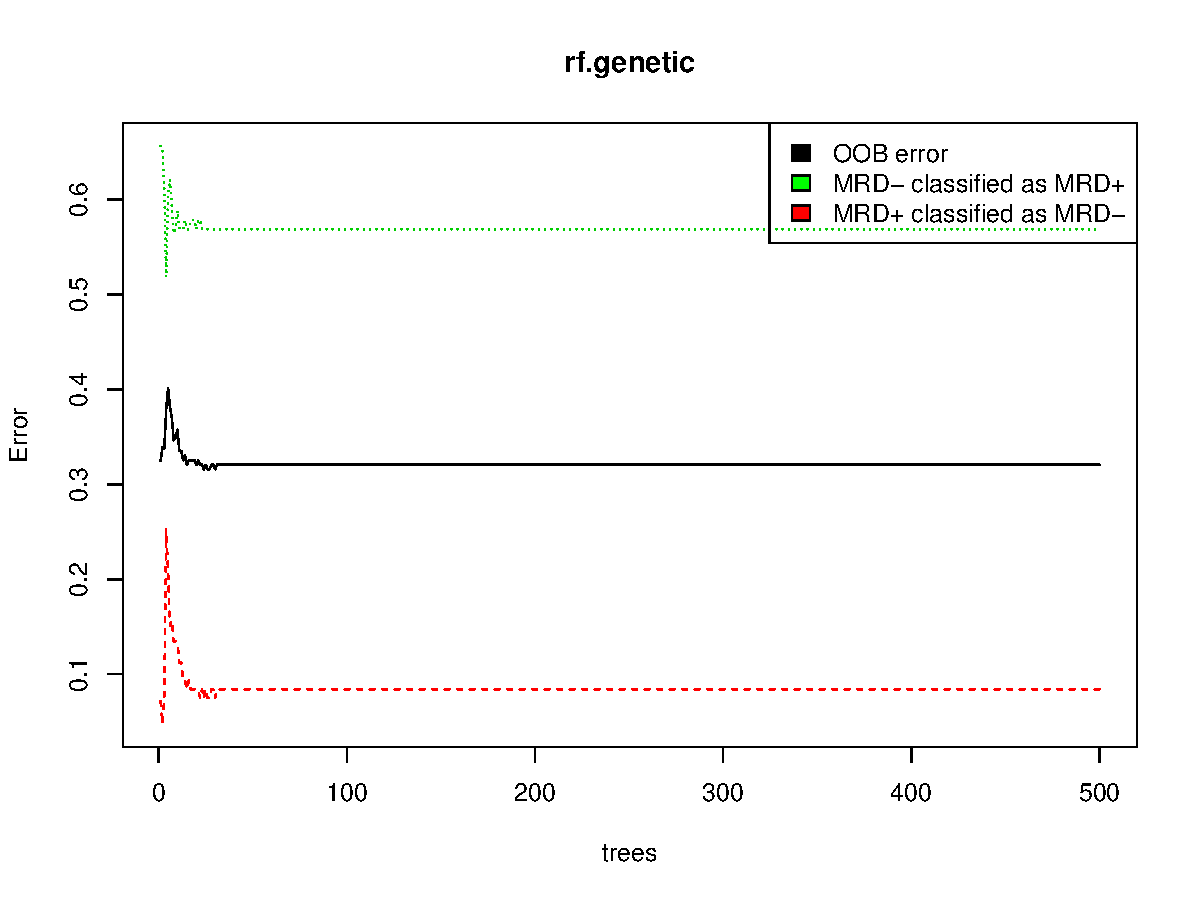
\includegraphics{HICF1_Finalreportv4-015}
\\
Conclusion: The number of trees does not seem to play an important role, 500 should be sufficient.
 
\subsubsection{Weighted class}
The focus of our study is to find predictors for "MRD positive"(to give him/her access to the more expensive drug). There is cost of increasing true negative findings (real "MRD positives") as we will also generate more false positive findings ("MRD negatives" that are classified as positives).\\
We can incorporate class weights into the random forest classifier, thus making it more sensitive to find MRD positives. The resulting errors are shown below:\\
